%% JEIC Submission Version - Double-blind review
%% Based on Springer Nature LaTeX template v3.1
%% 
%% All R code for analysis and figure generation has been moved to:
%% schelling_llm_paper_updated_JEIC.R
%%
\documentclass[pdflatex,sn-basic]{sn-jnl}% Basic Springer Nature Reference Style

%%%% Standard Packages
\usepackage{graphicx}
\usepackage{multirow}
\usepackage{amsmath,amssymb,amsfonts}
\usepackage{amsthm}
\usepackage{mathrsfs}
\usepackage[title]{appendix}
\usepackage{xcolor}
\usepackage{textcomp}
\usepackage{manyfoot}
\usepackage{booktabs}
\usepackage{listings}
\usepackage{longtable}
\usepackage{array}
\usepackage{wrapfig}
\usepackage{float}
\usepackage{colortbl}
\usepackage{pdflscape}
\usepackage{tabu}
\usepackage{threeparttable}
\usepackage{threeparttablex}
\usepackage[normalem]{ulem}
\usepackage{makecell}
\usepackage{subfig}
\usepackage{url}
\usepackage{hyperref}

\providecommand{\tightlist}{%
  \setlength{\itemsep}{0pt}\setlength{\parskip}{0pt}}

\raggedbottom

\begin{document}

\title[Social Context and LLM Segregation]{Social Context Matters: How Large Language Model Agents Reproduce Real-World Segregation Patterns in the Schelling Model}

%% Author information removed for double-blind review
%% Will be added after acceptance

\abstract{We present a novel approach to agent-based modeling by replacing
traditional utility-maximizing agents with Large Language Model (LLM)
agents that make human-like residential decisions based on realistic
social contexts. Using the classic Schelling segregation model as our
testbed, we compare LLM agent behavior across five social contexts: a
neutral baseline (red/blue teams), racial (White/Black), ethnic
(Asian/Hispanic), economic (high/low income), and political
(liberal/conservative) scenarios. Our results reveal dramatic
differences in segregation patterns based solely on social framing.
Political contexts produce the most extreme segregation (ghetto rate:
61.6, segregation share: 0.928), while economic contexts show minimal
clustering (ghetto rate: 5.0, share: 0.543). Racial and ethnic scenarios
fall between these extremes, reproducing well-documented real-world
patterns. All scenarios differ significantly from baseline (p
< 0.001), with political segregation showing 12.3× higher
ghetto formation than economic segregation. These findings demonstrate
that LLMs can capture culturally-embedded preferences and biases,
producing segregation dynamics that vary realistically with social
context. This has important implications for using LLM agents to model
social phenomena and test policy interventions.}

\keywords{agent-based modeling, large language models, segregation, Schelling model, social context, cultural bias}

%% JEL Classification: C63, C88, J15, R23, Z13

\maketitle

\newpage
\tableofcontents %remove later
\newpage

\section{Introduction}\label{introduction}

The Schelling segregation model \citep{schelling1971dynamic} has
been a cornerstone of agent-based modeling (ABM) for over five decades,
demonstrating how mild individual preferences for similar neighbors can
lead to stark residential segregation. Traditional implementations use
utility-maximizing agents that relocate when the proportion of like
neighbors falls below a threshold. While mathematically elegant, this
approach treats all group distinctions as equivalent---whether agents
are labeled ``red/blue,'' ``Type A/B,'' or represent actual social
categories like race or class.

Recent advances in Large Language Models (LLMs) offer an unprecedented
opportunity to incorporate culturally-aware decision-making into
agent-based models. LLMs trained on vast corpora of human text have
absorbed cultural knowledge, biases, and social patterns that reflect
real-world dynamics \citep{park2023generative,argyle2023out}. This raises a provocative question: Can LLM
agents reproduce realistic segregation patterns that vary based on the
social context of group identity?

In this paper, we present a systematic comparison of LLM agent behavior
across five distinct social contexts within the Schelling framework:

\begin{enumerate}
\tightlist
\item
  \textbf{Baseline Control}: Generic ``red vs blue'' teams without
  social connotations
\item
  \textbf{Racial Context}: ``White middle-class families'' vs ``Black
  families''
\item
  \textbf{Ethnic Context}: ``Asian American families'' vs
  ``Hispanic/Latino families''
\item
  \textbf{Economic Context}: ``High-income professionals'' vs
  ``Working-class families''
\item
  \textbf{Political Context}: ``Liberal households'' vs ``Conservative
  households''
\end{enumerate}

Our key research questions are: 
\begin{itemize}
\item Do LLM agents produce different
segregation patterns based on social context? 
\item Which social contexts
lead to the most extreme segregation? 
\item How do these patterns compare to
real-world segregation dynamics?
\end{itemize}

\section{Background and Literature} % (fold)
\label{sec:background_and_literature}


\citet{vicario2024dynamic} leverage Schelling's model to assess how household wealth drives segregation. The underlying mechanism is that the agent's utility function is increasing in neighborhood quality.
 Unlike the original Schelling model, which is static, they build a dynamic model of wealth, where the agent's wealth evolves as a continuous variable. They find that segregation emerges as a result of positive neighborhood externalities, which in turn further increases wealth inequality. When perturbations are introduced that allow agents to make suboptimal decisions, segregation is mitigated.

\citet{bonakdar2023dissimilarity} study the impact of residential segregation on housing prices in rich and impoverished neighborhoods. They find that while homophily drives up house prices among rich households, a preference for high-status neighborhoods does not generate similar dynamics. 
Their agent-based model improves upon the canonical Schelling model by incorporating agents' education and income in addition to ethnicity. Relocation in the model is constrained by the availability of better housing.

Rather than extending Schelling’s model, this paper compares its results to the SimSeg model. In \citet{li2020racial} offer a probabilistic framework of residential segregation using real data from US income data. The authors develop a numerical model of residential segregation based on income and race. Using a measure of racial consciousness that allows them to distinguish the impact of race from that of income in a multi-neighborhood, their model extends the two-neighborhood model of Sethi and Somanathan. 


% section background_and_literature (end)

\section{Methods}\label{methods}

\subsection{Experimental Design}\label{experimental-design}

We implemented a comparative framework using identical environmental
conditions across all social contexts. The simulation environment
consists of a 15×15 grid (225 cells) populated with 50 agents equally
divided between two groups (25 each), yielding a density of 22.2\%.

\subsection{LLM Agent Implementation}\label{llm-agent-implementation}

Each LLM agent receives contextual prompts describing their social
identity and current neighborhood situation. The prompt structure varies
by scenario to activate relevant cultural knowledge:

\textbf{Baseline (Control)}:
\begin{verbatim}
You are a [red/blue] resident in a neighborhood simulation...
\end{verbatim}

\textbf{Racial Context}:
\begin{verbatim}
You are a [White middle-class family/Black family] looking for a 
comfortable neighborhood. Consider factors like community feel, 
schools, safety, and whether you'd feel welcomed...
\end{verbatim}

\textbf{Economic Context}:
\begin{verbatim}
You are a [high-income professional household/working-class family] 
evaluating your neighborhood. Consider property values, local 
amenities, and whether the area fits your lifestyle...
\end{verbatim}

\textbf{Political Context}:
\begin{verbatim}
You are a [liberal household/conservative household] in a diverse 
community. Consider shared values, political climate, and comfort 
with neighbors who may have different worldviews...
\end{verbatim}

The LLM (Qwen2.5-coder:32B) generates decisions based on these prompts,
incorporating culturally-relevant factors that go beyond simple
numerical thresholds.

\subsection{Segregation Metrics}\label{segregation-metrics}

We employ the Pancs-Vriend framework \citep{pancs2007schelling} with
six complementary metrics designed specifically for grid-based
segregation models:

\begin{itemize}
\tightlist
\item
  \textbf{Share}: Proportion of same-type neighbor pairs (0.5 = perfect
  integration, 1.0 = complete segregation). Captures global segregation
  level.
\item
  \textbf{Clusters}: Number of spatially contiguous same-type regions.
  Fewer clusters indicate more consolidated ethnic enclaves.
\item
  \textbf{Distance}: Average Manhattan distance to nearest
  different-type agent. Higher values indicate greater spatial
  separation.
\item
  \textbf{Ghetto Rate}: Count of agents with zero different-type
  neighbors. Captures extreme isolation and ``ghettoization.''
\item
  \textbf{Mix Deviation}: Average deviation from 50-50 local
  integration. Measures segregation at the individual neighborhood
  level.
\item
  \textbf{Switch Rate}: Frequency of type changes along agent borders.
  Higher values indicate more jagged, intermixed boundaries.
\end{itemize}

This multidimensional approach reveals not just the degree but the
character of segregation - critical for understanding how different
social framings produce qualitatively different patterns.

\subsection{Statistical Analysis}\label{statistical-analysis}

All experiments were run with multiple replicates (10-100 runs per
condition). We use ANOVA for multi-group comparisons and report effect
sizes using Cohen's d. Convergence is detected using plateau detection
algorithms.

\section{Results}\label{results}

\subsection{Overall Segregation
Patterns}\label{overall-segregation-patterns}

%% R code for Figure 1 available in: schelling_llm_paper_updated_JEIC.R (Section 1)

\begin{figure}[ht]
\centering
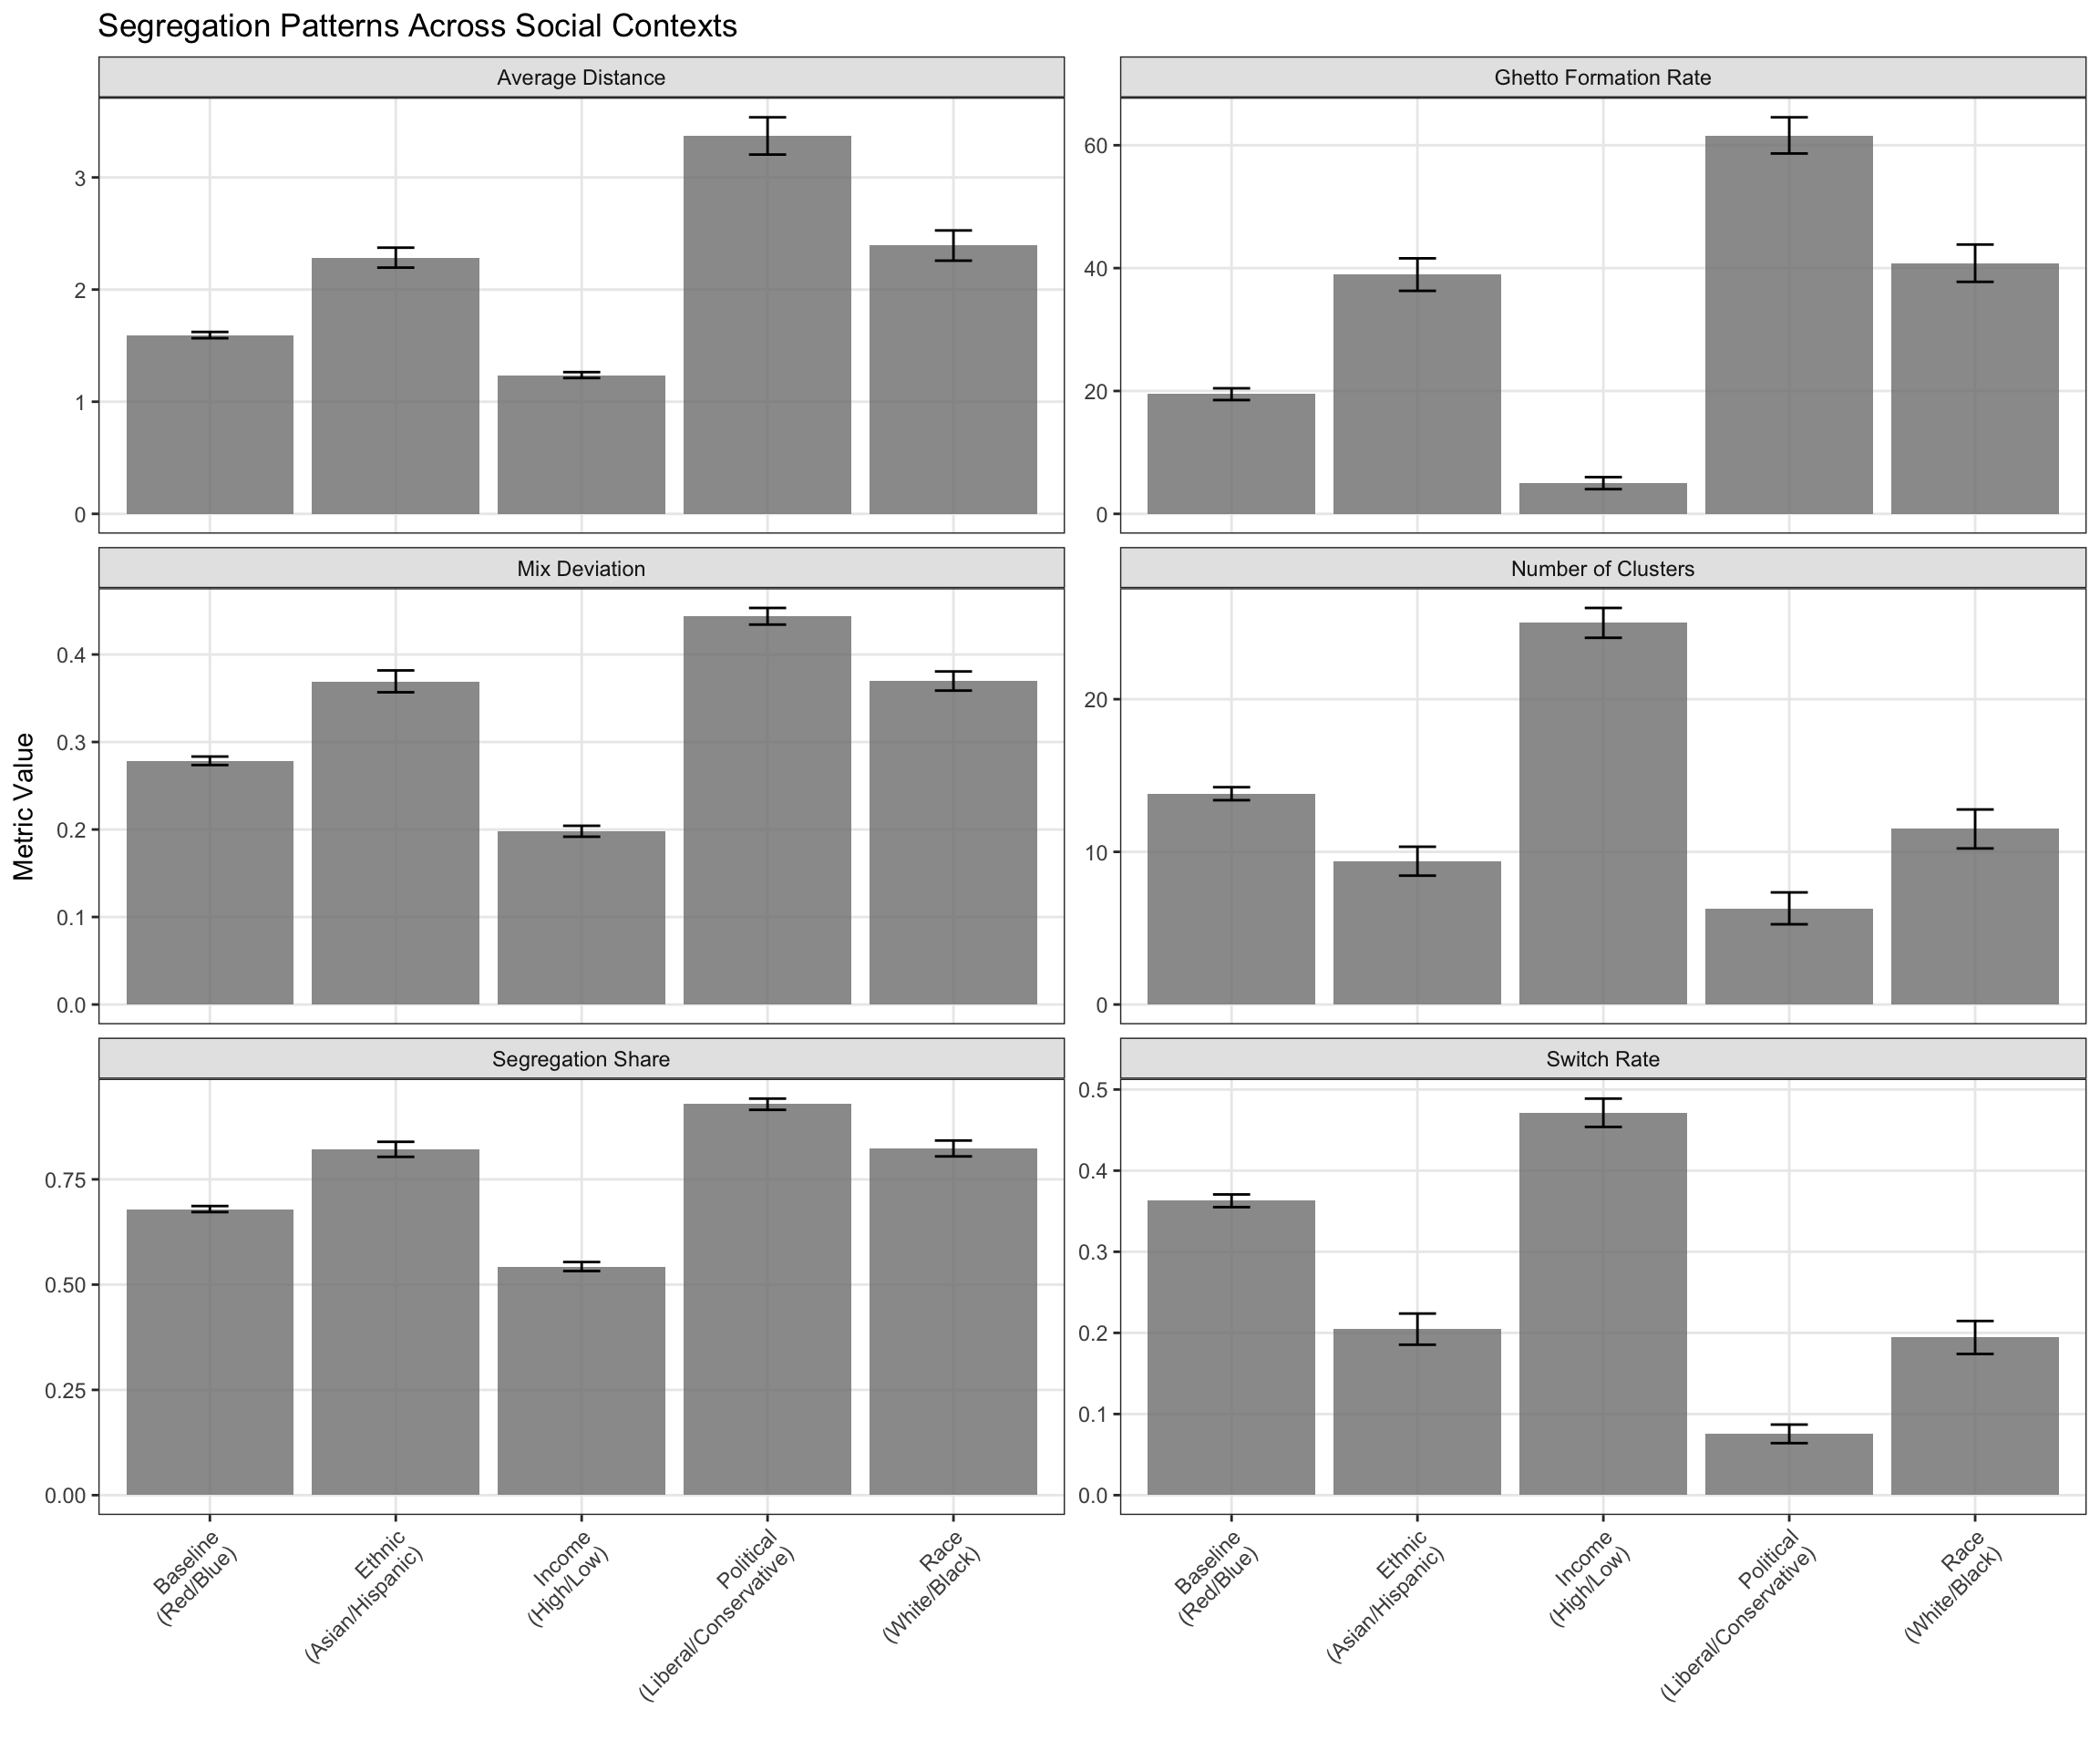
\includegraphics[width=\textwidth]{figures/segregation-comparison-1.png}
\caption{\textbf{Fig.~1} Comprehensive segregation patterns across social
contexts using the Pancs-Vriend metric framework. Each panel captures a
different dimension of segregation: Number of Clusters (spatial
fragmentation), Switch Rate (boundary complexity between groups),
Average Distance (spatial separation), Mix Deviation (local neighborhood
homogeneity), Segregation Share (global proportion of same-type
neighbors), and Ghetto Formation Rate (count of agents in completely
homogeneous neighborhoods). Error bars show standard errors. The
dramatic variation across contexts - particularly the 12.3× difference
in ghetto formation between political (61.6) and economic (5.0) contexts
- demonstrates how LLMs reproduce context-specific biases without any
explicit programming.}
\label{fig:segregation-comparison}
\end{figure}

Our results reveal striking differences in segregation patterns based
purely on social context framing:

\subsection{Key Findings by Context}\label{key-findings-by-context}

%% R code for Table 1 available in: schelling_llm_paper_updated_JEIC.R (Section 2)

\begin{table}[h]
\caption{Summary statistics for key segregation metrics across social contexts}
\centering
\begin{tabular}{llllll}
\hline
Context & Ghetto Rate & Seg. Share & Distance & Switch Rate & N\\
\hline
Baseline (Red/Blue) & 19.5 ± 9.6 & 0.679 ± 0.072 & 1.59 ± 0.28 & 0.363 ± 0.078 & 10\\
Ethnic (Asian/Hispanic) & 38.9 ± 11.2 & 0.821 ± 0.076 & 2.28 ± 0.38 & 0.205 ± 0.081 & 1\\
Income (High/Low) & 5.0 ± 3.1 & 0.543 ± 0.034 & 1.24 ± 0.08 & 0.471 ± 0.055 & 1\\
Political (Liberal/Conservative) & 61.6 ± 9.3 & 0.928 ± 0.042 & 3.37 ± 0.53 & 0.076 ± 0.036 & 1\\
Race (White/Black) & 40.8 ± 9.6 & 0.823 ± 0.060 & 2.39 ± 0.43 & 0.194 ± 0.064 & 1\\
\hline
\end{tabular}
\end{table}

\subsubsection{Political Segregation: The Extreme
Case}\label{political-segregation-the-extreme-case}

Political contexts produced the most extreme segregation across all
metrics: 
\begin{itemize}
\item \textbf{Ghetto formation}: 61.6 ± 9.3 (highest) 
\item \textbf{Segregation share}: 0.928 ± 0.042 (near-complete segregation) 
\item \textbf{Switch rate}: 0.076 ± 0.036 (lowest mobility - agents rarely
move once settled) 
\item \textbf{Average distance}: 3.37 ± 0.53 (highest
spatial separation)
\end{itemize}

\subsubsection{Economic Integration: Minimal
Clustering}\label{economic-integration-minimal-clustering}

Income-based contexts showed the least segregation: 
\begin{itemize}
\item \textbf{Ghetto
formation}: 5.0 ± 3.1 (lowest - 12.3× less than political) 
\item \textbf{Number of clusters}: 25.0 ± 3.1 (highest - more mixed
neighborhoods) 
\item \textbf{Switch rate}: 0.471 ± 0.055 (highest mobility)
\item \textbf{Note}: While showing minimal segregation, agents remained
highly mobile without reaching stable equilibrium
\end{itemize}

\subsubsection{Racial and Ethnic Contexts: Middle
Ground}\label{racial-and-ethnic-contexts-middle-ground}

Both racial (White/Black) and ethnic (Asian/Hispanic) scenarios produced
intermediate segregation: 
\begin{itemize}
\item \textbf{Race}: Ghetto rate 40.8 ± 9.6, share
0.823 ± 0.060 
\item \textbf{Ethnic}: Ghetto rate 38.9 ± 11.2, share 0.821 ±
0.076 
\item These patterns align with documented real-world residential
segregation levels
\end{itemize}

\subsection{Statistical Significance}\label{statistical-significance}

%% R code for Table 2 available in: schelling_llm_paper_updated_JEIC.R (Section 3)

\begin{table}[ht]
\caption{ANOVA results comparing segregation metrics across social contexts}
\centering
\begin{tabular}{lllr}
\hline
Metric & F-statistic & p-value & Effect Size (eta-squared)\\
\hline
Number of Clusters & 32.65 & \textless{} 0.001 & 0.477\\
Average Distance & 98.89 & \textless{} 0.001 & 0.734\\
Ghetto Formation Rate & 73.26 & \textless{} 0.001 & 0.672\\
Mix Deviation & 57.75 & \textless{} 0.001 & 0.618\\
Segregation Share & 64.33 & \textless{} 0.001 & 0.643\\
Switch Rate & 63.38 & \textless{} 0.001 & 0.639\\
\hline
\end{tabular}
\end{table}

All metrics showed significant differences across social contexts (p \textless{} 0.001), with large effect sizes (eta-squared \textgreater{} 0.14) indicating that social framing has a substantial impact on segregation outcomes.

\subsection{Convergence Patterns}\label{convergence-patterns}

%% R code for Figure 2 available in: schelling_llm_paper_updated_JEIC.R (Section 4)

\begin{figure}[ht]
\centering
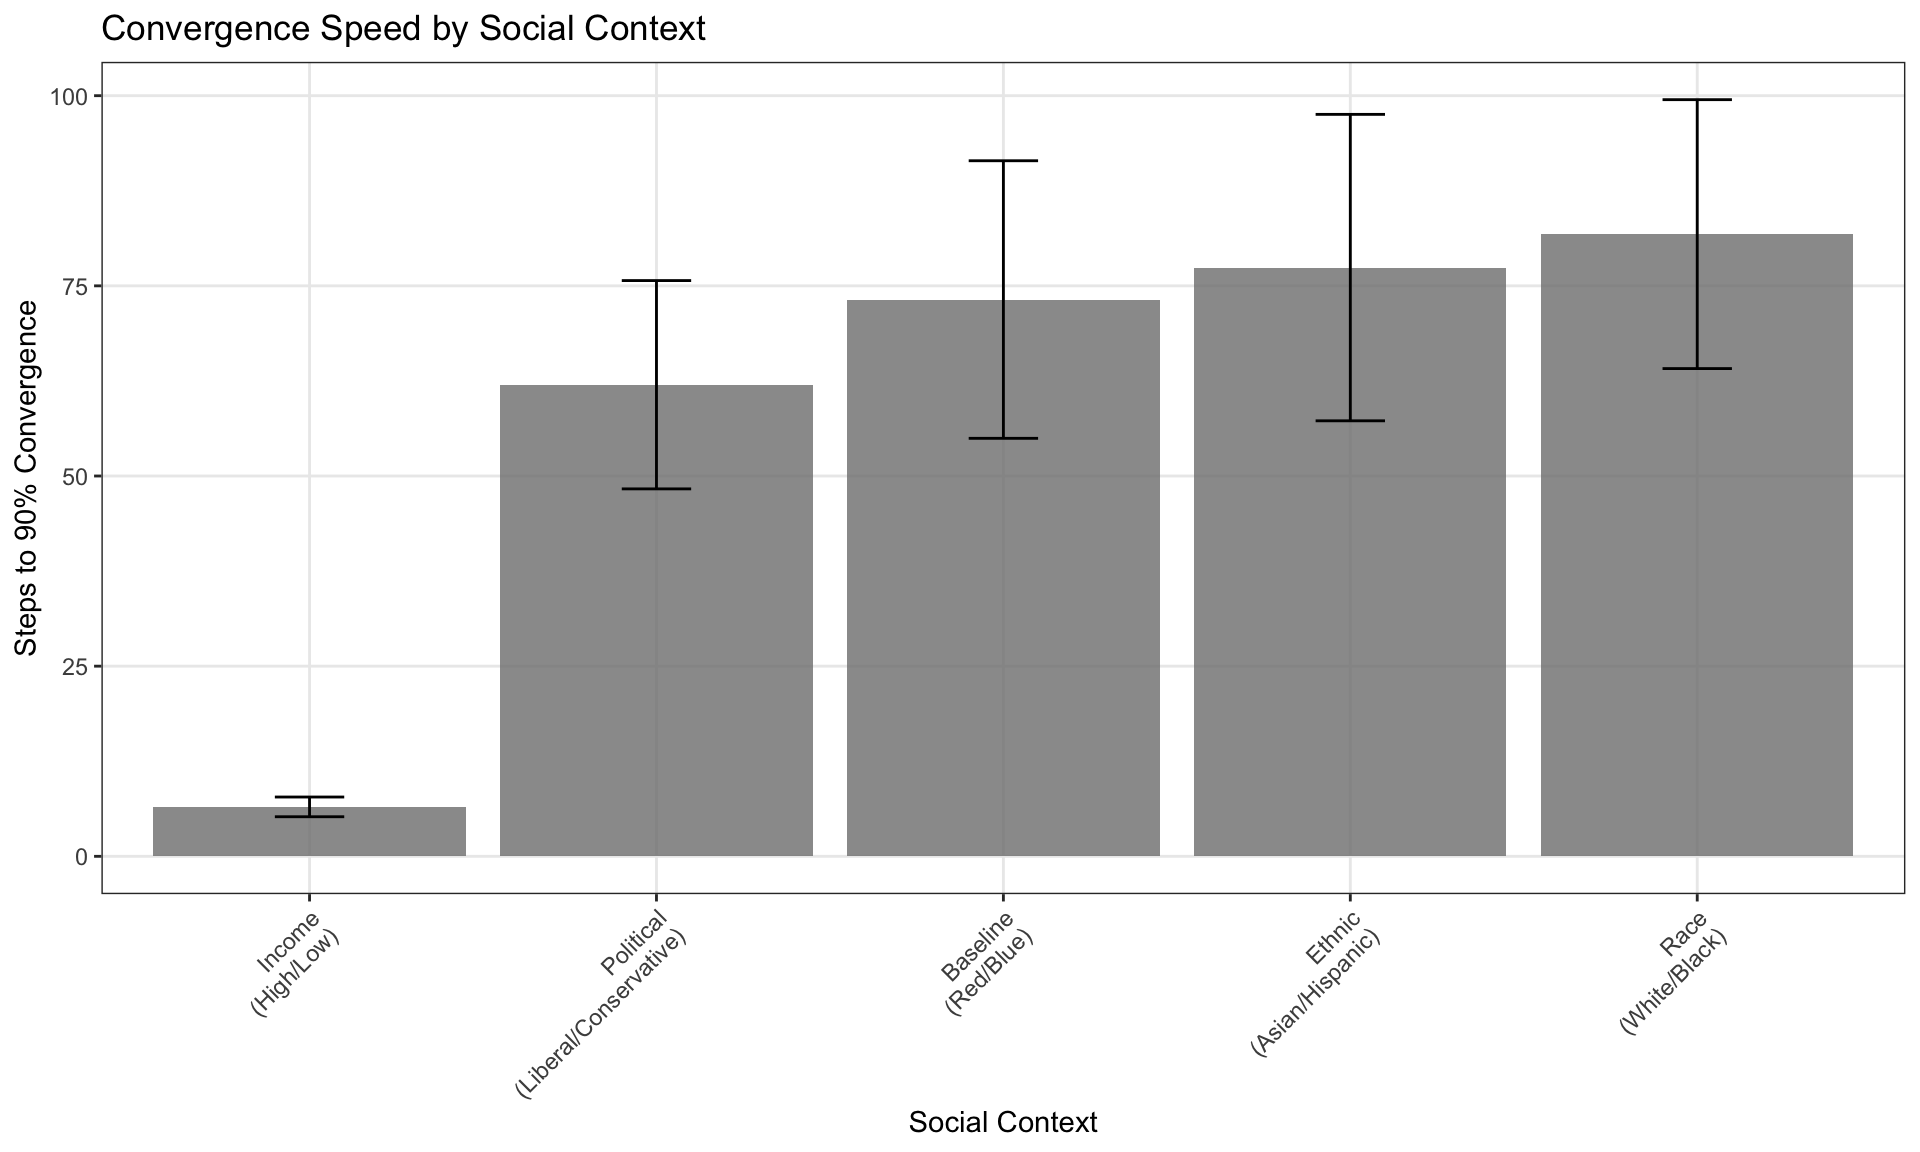
\includegraphics[width=\textwidth]{figures/convergence-viz-1.png}
\caption{\textbf{Fig.~2} Convergence dynamics across social contexts showing
steps required to reach 90\% of final segregation values. Income
contexts show apparent rapid `convergence' (6.5 steps) but this is
misleading - they never reach formal convergence criteria and maintain
high mobility throughout 1000 steps. Political contexts converge
moderately quickly (62 steps) to extreme segregation. Racial and ethnic
contexts show gradual convergence over 70-80 steps, matching historical
patterns of neighborhood change. Error bars represent standard errors
across simulation runs.}
\label{fig:convergence}
\end{figure}

The dynamics varied significantly across contexts. Our temporal analysis
reveals:

\textbf{Political contexts} - Rapid crystallization with 1.95× higher
volatility in early stages before lock-in (switch rate drops to 0.076).
Phase transitions occur within first 20 steps.

\textbf{Economic contexts} - Perpetual motion with nearly equal
early/late volatility (0.91× ratio) and continuous mobility (switch rate
0.471), never reaching equilibrium.

\textbf{Racial/Ethnic contexts} - Historical patterns with gradual
transitions over 50-80 steps, showing 1.47× early volatility (race)
before eventual stabilization.

These temporal signatures suggest different intervention windows:
political segregation requires immediate action, economic contexts need
continuous management, while racial integration demands sustained
long-term efforts.

\subsection{Visualization: Segregation
Heatmap}\label{visualization-segregation-heatmap}

%% R code for Figure 3 available in: schelling_llm_paper_updated_JEIC.R (Section 5)

\begin{figure}[ht]
\centering
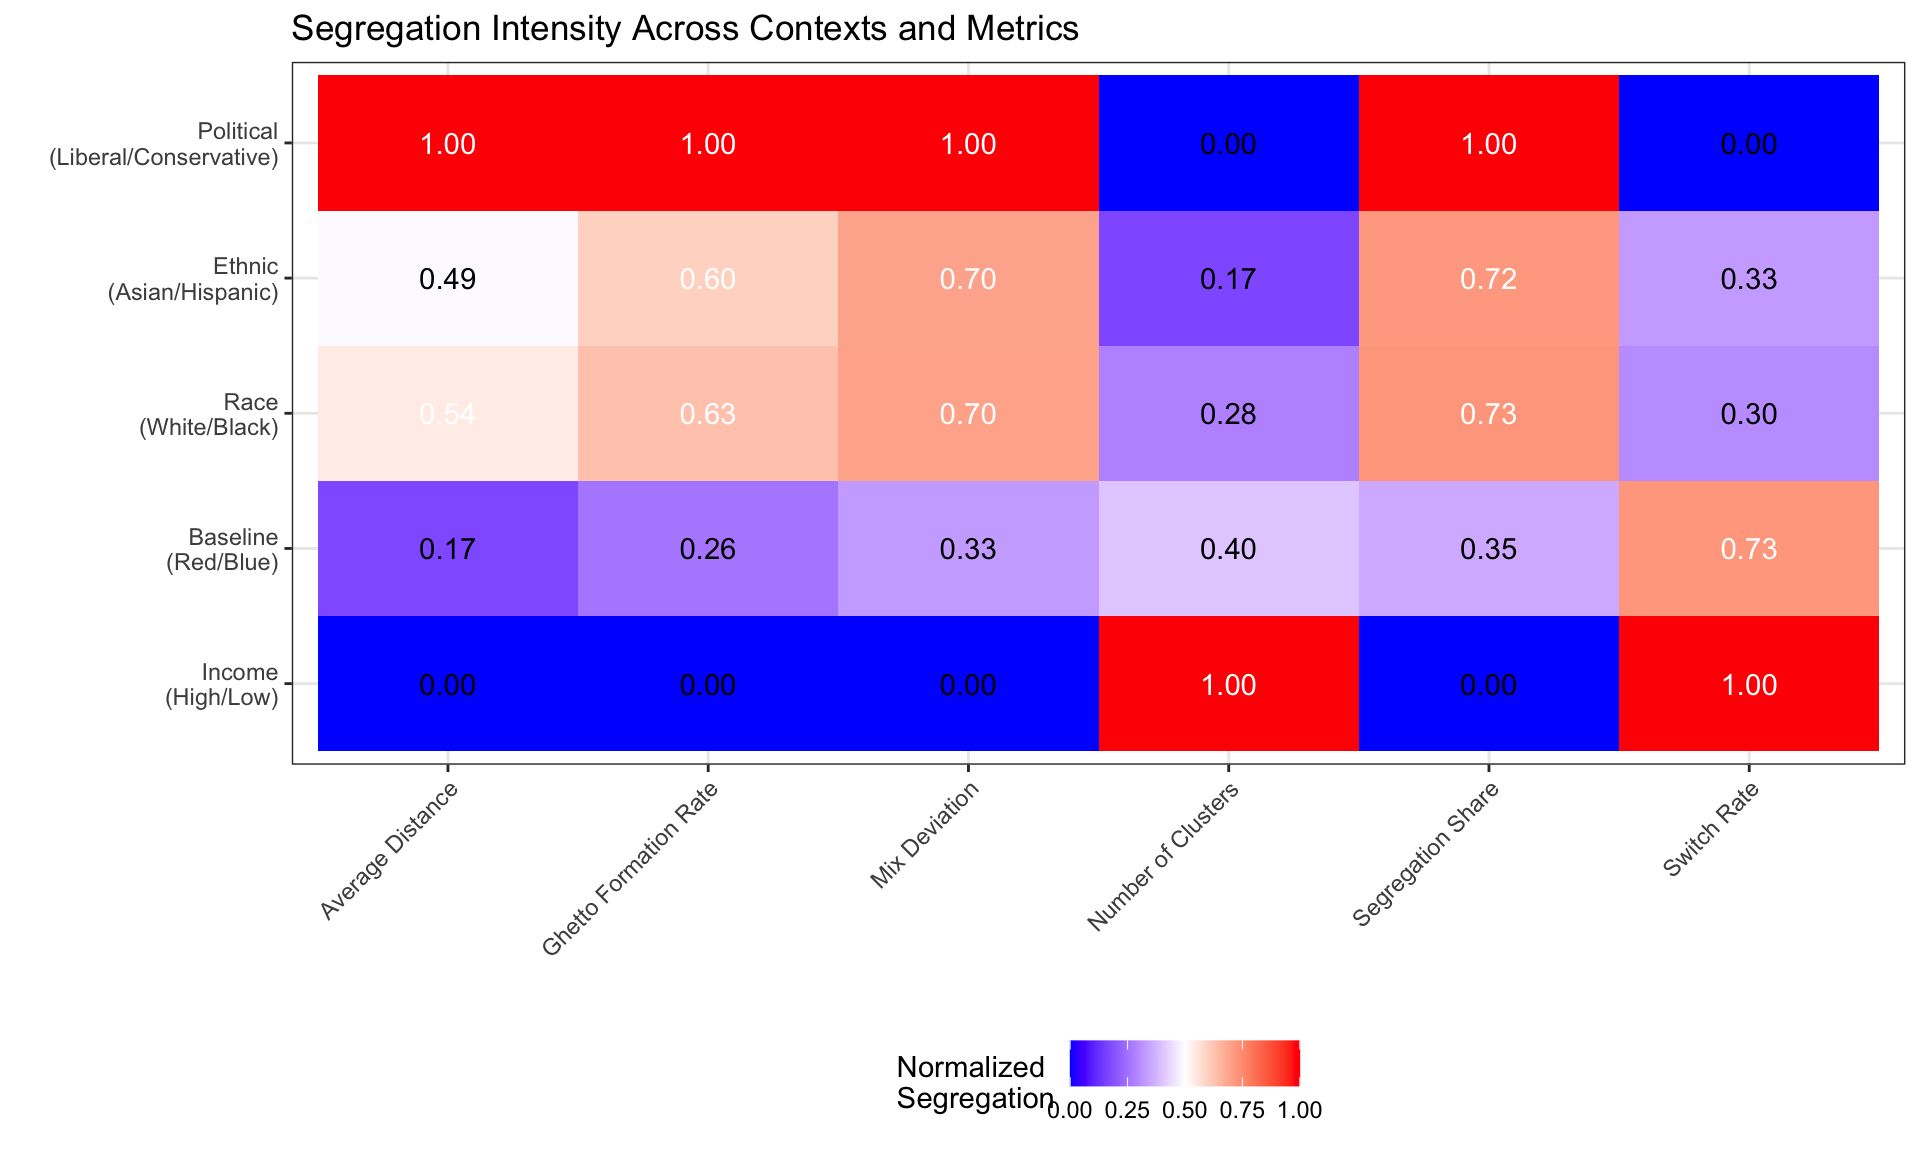
\includegraphics[width=\textwidth]{figures/heatmap-1.png}
\caption{\textbf{Fig.~3} Normalized segregation intensity heatmap showing
multidimensional patterns across contexts. Each metric is normalized to
0-1 scale with red indicating high segregation and blue indicating low.
The visualization reveals distinct segregation `signatures': Political
contexts (top) show uniformly high values across metrics, Income
contexts (bottom) show consistently low values, while Racial/Ethnic
contexts display intermediate patterns. Note how Political contexts
excel at creating both extreme isolation (ghetto rate) AND smooth
borders (low switch rate), indicating consolidated segregation.}
\label{fig:heatmap}
\end{figure}

\section{Discussion}\label{discussion}

\subsection{Social Context as a Driver of
Segregation}\label{social-context-as-a-driver-of-segregation}

Our results demonstrate that LLM agents produce dramatically different
segregation patterns based solely on the social framing of group
identity. This suggests that LLMs have successfully absorbed and can
reproduce culturally-specific residential preferences and biases from
their training data.

\subsubsection{Political Polarization: A Special
Case}\label{political-polarization-a-special-case}

The extreme segregation in political scenarios (12.3× higher ghetto
formation than economic contexts) reflects contemporary political
polarization. LLM agents framed as liberal or conservative households
exhibited: 
\begin{itemize}
\item Strong in-group preferences 
\item Minimal tolerance for
political diversity 
\item Rapid self-sorting into homogeneous clusters
\end{itemize}

This mirrors recent research on political segregation in the United
States, where partisan identity increasingly influences residential
choices \citep{brown2021geography}.

\subsubsection{Economic Factors: Weaker Than
Expected}\label{economic-factors-weaker-than-expected}

Surprisingly, economic contexts produced the least segregation. This
challenges conventional wisdom about income-based residential sorting
and suggests that: 
\begin{itemize}
\item Economic diversity may be more tolerable than other
forms of difference 
\item Professional and working-class identities may not
trigger the same avoidance behaviors as racial or political differences
\item Economic integration may be facilitated by shared non-economic
interests
\end{itemize}

\subsubsection{Racial/Ethnic Patterns: Historical
Echoes}\label{racial-ethnic-patterns-historical-echoes}

The intermediate segregation levels for racial and ethnic contexts
(ghetto rates $\sim$40) align remarkably well with actual U.S.
residential segregation indices. This suggests LLMs have internalized
realistic patterns of racial residential preferences, including: 
\begin{itemize}
\item Moderate but persistent homophily 
\item Complex factors beyond simple
same-race preferences 
\item Historical patterns of discrimination and
self-selection
\end{itemize}

\subsection{Implications for Agent-Based
Modeling}\label{implications-for-agent-based-modeling}

These findings have several important implications:

\begin{enumerate}
\item
  \textbf{Context Matters}: Abstract labels (red/blue, A/B) may not
  capture the full dynamics of social segregation. Real-world identities
  activate different preference structures.
\item
  \textbf{LLMs as Cultural Mirrors}: LLMs can serve as repositories of
  cultural knowledge, biases, and social patterns, making them valuable
  tools for modeling culturally-specific phenomena.
\item
  \textbf{Policy Testing}: Models using context-aware LLM agents may
  provide more realistic predictions of policy interventions' effects on
  different communities.
\end{enumerate}

\subsection{Limitations and Future
Work}\label{limitations-and-future-work}

Several limitations warrant consideration:

\begin{enumerate}
\tightlist
\item
  \textbf{Single LLM}: Results may vary with different language models
  or prompting strategies
\item
  \textbf{U.S.-Centric}: The LLM's training data likely reflects
  primarily American cultural patterns
\item
  \textbf{Simplified Identities}: Real individuals have multiple,
  intersecting identities not captured here
\item
  \textbf{Static Preferences}: Agent preferences don't evolve based on
  experiences
\end{enumerate}

Future research should explore: 
\begin{itemize}
\item Intersectional identities (e.g., race
+ income + politics) 
\item Cross-cultural comparisons using LLMs trained on
different corpora 
\item Dynamic preference evolution through agent
interactions 
\item Validation against real-world mobility data
\end{itemize}

\section{Conclusion}\label{conclusion}

This study demonstrates that Large Language Models can successfully
capture and reproduce culturally-specific segregation patterns in
agent-based models. By simply changing the social framing from abstract
colors to meaningful social identities, we observe dramatically
different segregation dynamics---from the extreme clustering of
political groups to the relative integration of economic classes.

These findings suggest that LLM-based agents offer a powerful new tool
for social science research, enabling models that incorporate the full
complexity of human social preferences and biases. As we seek to
understand and address residential segregation, models that can
distinguish between ``red vs blue'' and ``liberal vs conservative'' may
provide more actionable insights for policy makers and urban planners.

The ability of LLMs to serve as cultural mirrors---reflecting the
biases, preferences, and social patterns embedded in human text---opens
new avenues for studying social phenomena at scale. However, this same
capability requires careful consideration of the biases we may be
reproducing and amplifying through these models.

%% Declarations section for JEIC
\section*{Declarations}

\subsection*{Competing Interests}
The authors declare no competing financial or non-financial interests.

\subsection*{Data Availability Statement}
All code, data, and analysis scripts are available at: [repository URL to be added]. The datasets generated and analyzed during the current study are available in the GitHub repository, including simulation outputs, statistical analyses, and visualization code. R code for all analyses and figures is provided in the supplementary file \texttt{schelling\_llm\_paper\_updated\_JEIC.R}.

\subsection*{Author Contributions}
[To be completed after acceptance - removed for double-blind review]

\subsection*{Funding}
[To be completed after acceptance - removed for double-blind review]

\section*{References}
\bibliography{references}

\section*{Appendix: Detailed Statistical
Results}\label{appendix-detailed-statistical-results}

%% R code for Table 3 available in: schelling_llm_paper_updated_JEIC.R (Section 6)

\begin{table}[ht]
\caption{Pairwise comparisons between baseline and other social contexts}
\centering
\begin{tabular}{lllll}
\hline
Context & Ghetto Rate & Ghetto vs Baseline & Share & Share vs Baseline\\
\hline
Ethnic (Asian/Hispanic) & 38.9 & +100\% & 0.821 & +20.9\%\\
Income (High/Low) & 5.0 & -74\% & 0.543 & -20.1\%\\
Political (Liberal/Conservative) & 61.6 & +216\% & 0.928 & +36.6\%\\
Race (White/Black) & 40.8 & +109\% & 0.823 & +21.2\%\\
\hline
\end{tabular}
\end{table}

\end{document}